\chapter{Servidor Web com NodeJS}\label{cap:cap_03}

\begin{flushright}
	\textit{
		As raízes do estudo são amargas, \\ mas seus frutos são doces.
	} \\
	\textbf{Aristóteles}
\end{flushright}

Ao acessar e visualizar uma página em seu navegador, como, por exemplo \url{https://www.ifms.edu.br}, você está fazendo uma solicitação (request) a outro computador na rede (ou internet), que em resposta (response), fornece a você a página Web. O computador que está se comunicando por meio da sua solicitação executa uma aplicação que é o \textbf{servidor Web}. Um servidor Web recebe solicitações HTTP de um \textbf{cliente}, como seu navegador, e fornece uma resposta HTTP, como uma página HTML.

O \textbf{Node.js} permite que os desenvolvedores utilizem o JavaScript para escrever o código do lado do servidor (Server-Side), embora ele seja tradicionalmente usado no navegador para escrever o código do lado do cliente (Client-Side). Assim, vamos aprender como desenvolver servidores Web usando o módulo http que está incluído no Node.js que poderá retornar dados em JSON, arquivos CSV e páginas Web em HTML.

\section{Criando um servidor HTTP básico}

Para iniciarmos a configuração vamos criar um servidor que retorna um texto sem formatação ao usuário. Primeiro, precisamos configurar um ambiente de programação acessível para fazer nossos exercícios. Para tanto, vamos criar e acessar uma pasta chamada \textbf{primeiro-servidor}:

\begin{minted}[frame=single,framesep=10pt,breaklines,linenos,tabsize=2,autogobble]{javascript}
mkdir primeiro-servidor
cd primeiro-servidor
\end{minted}

Dentro do diretório vamos criar um arquivo com o nome de \textbf{index.js} e nele iniciaremos as primeiras linhas para a implementação do nosso servidor HTTP. Começaremos carregando o módulo \textbf{http}, padrão em todas as instalações do Node.js. Adicione a linha seguinte ao \textbf{index.js}:

\begin{minted}[frame=single,framesep=10pt,breaklines,linenos,tabsize=2,autogobble]{javascript}
const http = require("http");
\end{minted}

Nosso próximo passo definiremos duas constantes, o \textbf{host} e a \textbf{porta} em que nosso servidor se associará. O \textbf{host} nada mais é do que o ``endereço'' que faremos o acesso ao servidor e a \textbf{porta} pode ser qualquer número entre 1024 até 40.000. Contudo, por padrão, vamos usar a porta 8080.

\begin{minted}[frame=single,framesep=10pt,breaklines,linenos,tabsize=2,autogobble]{javascript}
const http = require("http");

const host = 'localhost';
const porta = 8080;
\end{minted} 

Como mencionado anteriormente, os servidores Web aceitam solicitações de navegadores e de outros clientes. Podemos interagir com um servidor Web ao digitar um nome de domínio. O valor \textbf{localhost} é um endereço privado especial que os computadores utilizam para se referir a eles mesmos. Normalmente, ele é equivalente ao endereço \textbf{IP interno 127.0.0.1} e está disponível apenas para o computador local, ou seja, não está disponível para nenhuma rede local da qual participamos ou para a Internet. Por fim, definimos a porta, que é o número que representa o ``local'' no computador onde o servidor está sendo executado. 

Ao vincularmos nosso \textbf{servidor} a este \textbf{host} e \textbf{porta}, conseguiremos acessar nosso servidor ao visitarmos http://localhost:8080 em um navegador local.

Vamos adicionar uma função especial que em Node.js, chamamos \textbf{resposta}. Esta função foi criada para processar uma solicitação HTTP de entrada e retornar uma resposta HTTP. A função deve ter dois argumentos: um \textbf{objeto de solicitação} e um \textbf{objeto de resposta}. O objeto de solicitação capta todos os dados da solicitação HTTP que chegam. O objeto de resposta é usado para devolver respostas HTTP para o servidor.

\begin{minted}[frame=single,framesep=10pt,breaklines,linenos,tabsize=2,autogobble]{javascript}
const http = require("http");
const host = 'localhost';
const porta = 8080;

const resposta = function (req, res) {
	res.writeHead(200);
	res.end("Meu primeiro servidor!!!");
};
\end{minted}

Por fim, podemos criar nosso servidor e usar nossa função de resposta:

\begin{minted}[frame=single,framesep=10pt,breaklines,linenos,tabsize=2,autogobble]{javascript}
const http = require("http");
const host = 'localhost';
const porta = 8080;

const resposta = function (req, res) {
	res.writeHead(200);
	res.end("Meu primeiro servidor!!!");
};

const server = http.createServer(resposta);
server.listen(porta, host, function() {
	console.log(`Servidor sendo executado em http://${host}:${porta}`);
});
\end{minted}

Caso deseje disponibilizar o acesso para todos na rede, basta adicionar o endereço \textbf{0.0.0.0} no lugar no \textbf{localhost}.

\begin{minted}[frame=single,framesep=10pt,breaklines,linenos,tabsize=2,autogobble]{javascript}
	const http = require("http");
	const host = '0.0.0.0';
	const porta = 8080;
	
	const resposta = function (req, res) {
		res.writeHead(200);
		res.end("Meu primeiro servidor!!!");
	};
	
	const server = http.createServer(resposta);
	server.listen(porta, host, function() {
		console.log(`Servidor sendo executado em http://${host}:${porta}`);
	});
\end{minted}

\section{Retornando tipos diferentes de conteúdo}

Para podermos retorna uma categoria de conteúdo diferente do que é apresentado, devemos adicionar o tipo de conteúdo que queremos. Para tanto, vamos adicionar um cabeçalho informado ao navegador a forma com que ele deve tratar o conteúdo que chega-lhe por meio da resposta.

\begin{minted}[frame=single,framesep=10pt,breaklines,linenos,tabsize=2,autogobble]{javascript}
res.setHeader("Content-Type", "text/html");
res.end(`<html><body><h1>This is HTML</h1></body></html>`);
\end{minted}

O código completo, adicionado indentação e tags para inserir css,  ficará da seguinte forma. 

\begin{minted}[frame=single,framesep=10pt,breaklines,linenos,tabsize=2,autogobble]{javascript}
const http = require("http");
const host = '0.0.0.0';
const porta = 8080;

const resposta = function (req, res) {
	res.setHeader("Content-Type", "text/html");
	res.writeHead(200);
	res.end(`
		<html>
			<head>
				<style>
					body {
						background: #000
					}
				</style>
			</head>
				<body>
					<h1>This is HTML</h1>
				</body>
		</html>
	`);
};

const server = http.createServer(resposta);
server.listen(porta, host, function() {
	console.log(`Servidor sendo executado em http://${host}:${porta}`);
});
\end{minted}

\section{Gerenciador de pacotes para Node.js}

Existem diversas formas para instalar pacotes em diversas linguagem e ambientes de desenvolvimento. A mais utilizada é por meio da utilização de aplicativos específicos, conhecidos como \textbf{gerenciadores de pacotes}. \textbf{Pacotes} são arquivos que contém bibliotecas e seus arquivos de configuração, como também, todas as dependências (outros pacotes) requeridos para a instalação.

Várias linguagem possuem seus respectivos gerenciadores, e, no caso do Nodejs os mais usados são o \textbf{Yarn} e o \textbf{NPM}. O Yarn é um gerenciador de pacotes para Node.js que se concentra em velocidade, segurança e consistência. Ele foi criado originalmente para resolver alguns problemas com o popular gerenciador de pacotes NPM. Embora os dois gerenciadores de pacotes tenham convergido em termos de desempenho e recursos, o Yarn continua popular, especialmente no mundo do desenvolvimento React.

\subsection{Usando o Yarn}\label{usando_yarn}

O Yarn tem muitos subcomandos, mas precisamos apenas de alguns para começar. Vejamos os primeiros subcomandos desejamos usar.

\begin{minted}[frame=single,framesep=10pt,breaklines,linenos,tabsize=2,autogobble]{javascript}
	yarn --help // Mostra a ajuda
	yarn install --help // Mostra a ajuda para os comandos de instalação
	yarn init // Inicia um projeto
	yarn add [pacote] // Instala um pacote
	yarn add [pacote] --dev // instala um pacote em desenvolvimento
	yarn install // Instala as dependências
 \end{minted}

\subsection{Iniciando um novo projeto}

Para iniciar um projeto criamos um diretório e, interno a ele, executamos o comando os seguintes comandos: 

\begin{minted}[frame=single,framesep=10pt,breaklines,linenos,tabsize=2,autogobble]{javascript}
	mkdir nome-projeto 
	cd nome-projeto
	yarn init // ou como recomendo o npm init
\end{minted}

Após o comando o Yarn executará algumas perguntas, Responda com os dados desejados e por fim será gerado um arquivo \textbf{package.json}. O package.json é um arquivo de configuração utilizado para estipular e configurar \textbf{dependências} do seu projeto (quais outros pacotes ele vai precisar para ser executado) e \textbf{scripts} automatizados. 

Agora, para adicionar uma dependência, vamos ao site do Yarn \url{https://yarnpkg.com/} ou Npm \url{https://www.npmjs.com/} e buscar o pacote que desejamos. No caso, vamos usar um para validar CPFs, o qual pode ser encontrado em \url{https://yarnpkg.com/package/cpf}.

Seguindo a documentação, para instalarmos o pacote devemos executar o seguinte comando:

\begin{minted}[frame=single,framesep=10pt,breaklines,linenos,tabsize=2,autogobble]{javascript}
	yarn add cpf
\end{minted}

Assim, "magicamente", o pacote é instalado em nosso computador dentro de um diretório no projeto chamado \textbf{Node Modules} e o arquivo \textbf{package.json} e atualizado com a nova dependência, inclusive, em sua última versão. 

\begin{minted}[frame=single,framesep=10pt,breaklines,linenos,tabsize=2,autogobble]{javascript}
	...
	"dependencies": {
		"cpf": "^2.0.1"
	}
	...
\end{minted}

O \textbf{Node Modules} é um diretório que pode ser deletado e recriado quando necessário. Para tanto, devemos apenas executar o comando abaixo que todas as dependências serão reinstaladas. 

\begin{minted}[frame=single,framesep=10pt,breaklines,linenos,tabsize=2,autogobble]{javascript}
	yarn install // ou apenas yarn
\end{minted}

Para utilizar o pacote instalado, será necessário verificar a documentação. Contudo, o instalado anteriormente, pode ser usado da seguinte forma. Em um arquivo \textbf{index.js} adicione os seguintes comandos: 

\begin{minted}[frame=single,framesep=10pt,breaklines,linenos,tabsize=2,autogobble]{javascript}
	const CPF = require('cpf');
	console.log(CPF.format('11144477735'))
	console.log(CPF.isValid('111.444.777-35'));
\end{minted}

Após isso podemos executar o comando \textbf{node index.js} ou adicionar um executado no arquivo \textbf{package.json} da seguinte forma:

\begin{minted}[frame=single,framesep=10pt,breaklines,linenos,tabsize=2,autogobble]{javascript}
	"scripts": {
		"start": "node index.js",
		"test": "echo \"Error: no test specified\" && exit 1"
	}
\end{minted}

Por fim, executar o comando \textbf{yarn start} que obteremos a seguinte saída:

\begin{minted}[frame=single,framesep=10pt,breaklines,linenos,tabsize=2,autogobble]{javascript}
	$ yarn start
	yarn run v1.22.19
	$ node index.js
	
	111.444.777-35
	true
	
	Done in 1.02s.
\end{minted}

Agora, para executarmos o próximo exercício, vamos usar um pacote chamado \textbf{nodemon}. Para tanto, instale o pacote \textbf{yarn add nodemon --dev} e observe como foi modificado o \textbf{package.json}. Por fim, adicione o seguinte comando ao \textbf{script} do seu arquivo para que, a cada mudança feita, o servidor seja reiniciado. 

\begin{minted}[frame=single,framesep=10pt,breaklines,linenos,tabsize=2,autogobble]{javascript}
	"scripts": {
		"start": "nodemon index.js"
	}
\end{minted}

\section{Exercício de fixação}

\begin{enumerate}[leftmargin=1.7cm]
	\setlength\itemsep{0em}
	\item \label{questao_1} Crie uma página pessoal contendo informações sobre você, tais como, data de nascimento, nome completo, endereço, email, etc. Formate ela usando CSS e disponibilize na rede para que outros possam acessá-la. 
	
	\item Usando comentários, explique, com detalhes, o que faz cada linha do código criado no exercício \ref{questao_1}. 
	
	\item Liste, ao menos, 5 pontos negativos relacionados ao desenvolvimento do código da questão \ref{questao_1}. Pense em pontos que dificultaram o desenvolvimento e que podem ser melhorados.  
	
	\item Baseando-se nas explicações dadas em aula, explique o que é um \textbf{Host} e o que é uma \textbf{Porta}. Caso deseje, use analogias para reforçar sua resposta.
\end{enumerate}

\section{Padrão em design de software MVC}

MVC (Model-View-Controller) é um padrão em design de software comumente usado para implementar \textbf{interfaces} de usuário, \textbf{dados} e \textbf{lógica de controle}. Ele enfatiza uma separação entre a lógica de negócios do software e a exibição. Esta ``separação de interesses'' proporciona uma melhor divisão do trabalho e uma melhor manutenção.

As três partes do padrão de projeto de software MVC podem ser descritas da seguinte forma:

\begin{itemize}[leftmargin=1.7cm]
	\setlength\itemsep{0em}
	\item \textbf{Modelo}: Gerencia dados e lógica de negócios.
	\item \textbf{View}: lida com layout e exibição.
	\item \textbf{Controlador}: roteia comandos para as peças do modelo e da visualização.
\end{itemize}

\begin{figure}[H]
	\centering
	\caption{MVC}
	\frame{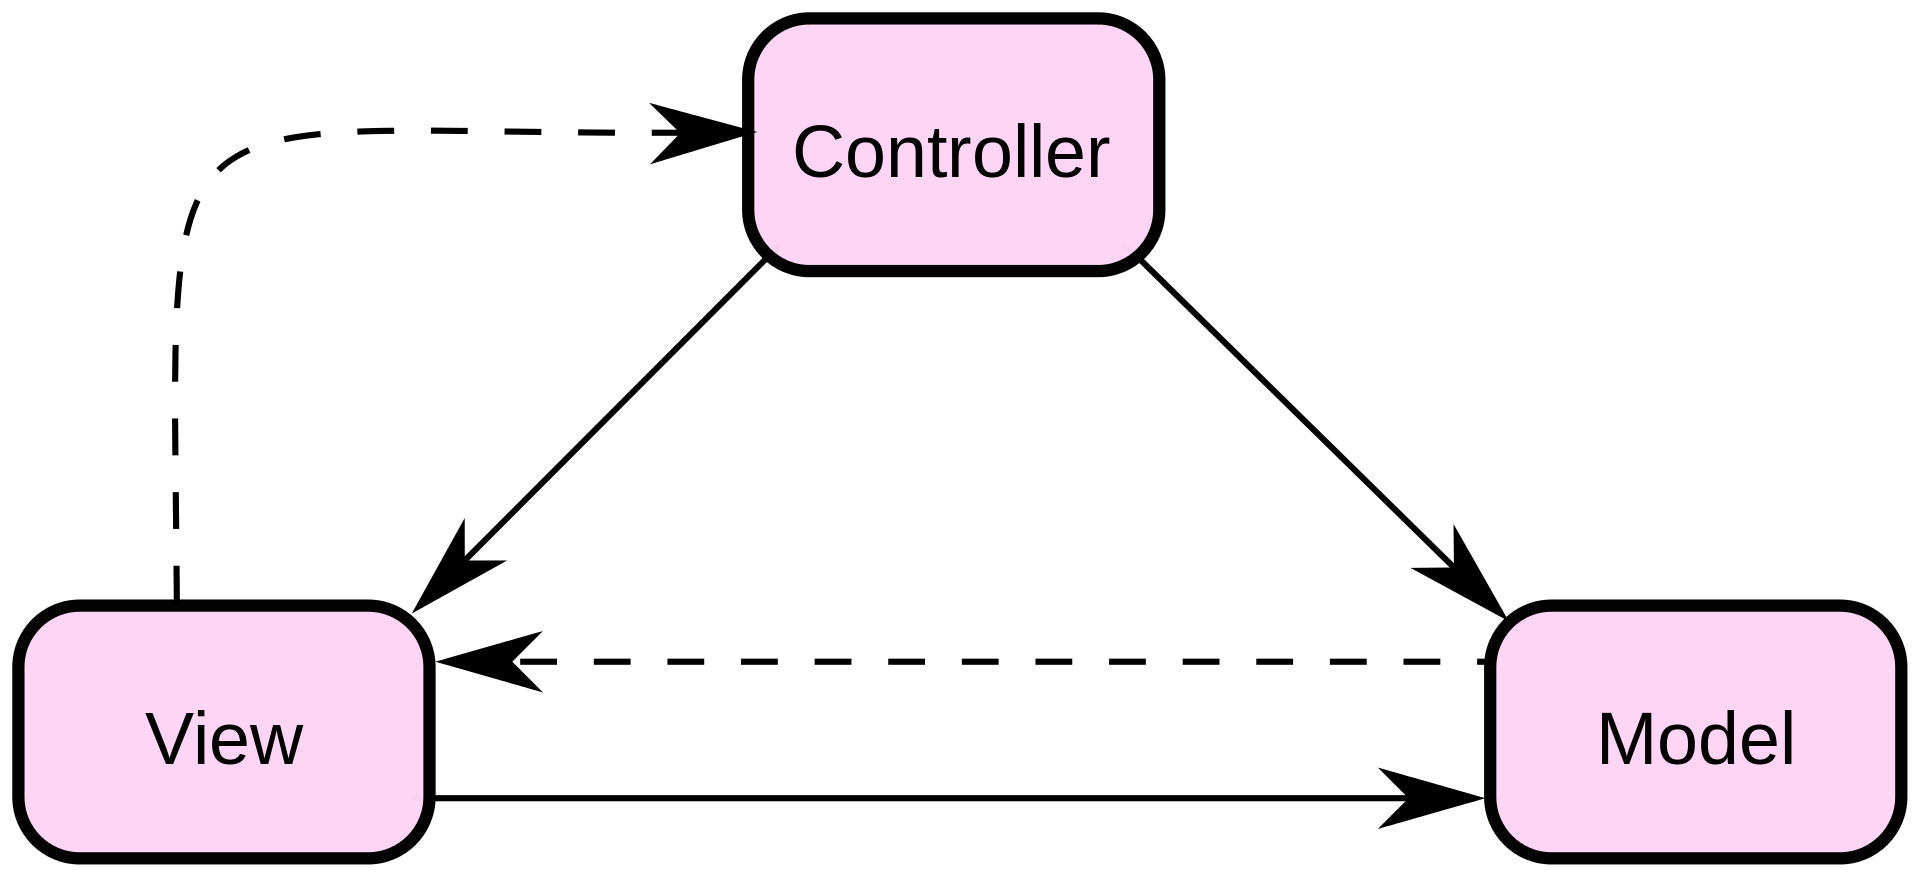
\includegraphics[scale=0.15]{imagens/mvc.png}}
	\legend{Fonte: \url{https://pt.wikipedia.org/wiki/MVC}}
	\label{fig:mvc}
\end{figure}

\subsection{O que faz cada camada?}

As camadas do \textbf{Padrão de Design MVC} possuem cada uma sua responsabilidade. Tais responsabilidades são listas abaixo:

\begin{itemize}[leftmargin=1.7cm]
	\setlength\itemsep{0em}
	\item \textbf{Controladores - Controllers}: Um Controller representa as classes que conectam o modelo e a visão e é usado para comunicação entre as classes no \textbf{modelo} e na \textbf{visão}.
	\item \textbf{Visualizações - Views}: Uma View é uma coleção de classes que representam os elementos na interface do usuário (todas as coisas que o usuário pode ver e responder na tela, como botões, caixas de exibição e assim por diante)
	\item \textbf{Modelos - Models}: Um modelo representa a estrutura lógica subjacente de dados em um aplicativo de software e a classe de alto nível associada a ele. Este modelo de objeto não contém nenhuma informação sobre a interface do usuário.
\end{itemize}

Assim, para podermos usar a estrutura MVC em nossos projetos, devemos usar uma ferramenta que possibilite as conexões listas acima. Para tanto, vamos usar um em específico, o \textbf{ExpressJS}.

\section{Express Web Framework}

Alguns problemas surgem quando vamos desenvolver. No exercício anterior, para criarmos uma página simples, conseguimos resolver facilmente. Contudo, caso queiramos uma organização ou apenas criar uma página a tarefa é bem mais complicada. Assim, para resolver esses problemas, que não são apenas nossos, mas comuns durante o desenvolvimento profissional, foram criadas ferramentas cujo objetivo é facilitar a codificação e reduzir a repetição de código. Uma dessas é o \textbf{Framework ExpressJS}. 

\begin{citacao}
	Assim um \textbf{Framework} tem como principal objetivo resolver problemas recorrentes com uma abordagem genérica, permitindo ao desenvolvedor focar seus esforços na resolução do problema em si, e não ficar reescrevendo software \cite{mozzila}. 
\end{citacao}

Express é um popular framework web estruturado, escrito em JavaScript que roda sobre o ambiente NodeJS em tempo de execução. Este módulo explica alguns dos principais benefícios deste framework, como configurar o seu ambiente de desenvolvimento e como executar tarefas comuns de desenvolvimento e implantação da web.

\subsection{Instalando o ExpressJS}

Para realizar a instalação do ExpressJS vamos seguir o Guia presente em \url{https://expressjs.com/pt-br/starter/installing.html}. Assumindo que já tenha instalado o Node.js, crie um diretório para conter o seu aplicativo, e torne-o seu diretório ativo iniciando um projeto usando o \textbf{Yarn} como feito em \ref{usando_yarn}.

Para instalar o express usando o seguinte comando:

\begin{minted}[frame=single,framesep=10pt,breaklines,linenos,tabsize=2,autogobble]{bash}
	yarn add express
\end{minted}

\subsection{Exemplo Hello World}
Para nosso primeiro exemplo vamos continuar usando o Guia citado anteriormente \url{https://expressjs.com/pt-br/starter/hello-world.html}. No diretório criado crie um arquivo chamado \textbf{index.js} e inclua o seguinte código:

\begin{minted}[frame=single,framesep=10pt,breaklines,linenos,tabsize=2,autogobble]{javascript}
	const express = require('express')
	const app = express()
	const port = 3000
	
	app.get('/', (req, res) => {
		res.send('<h1>Hello World!</h1>')
	})
	
	app.listen(port, () => {
		console.log(`Servidor escutando na porta ${port}`)
	})
\end{minted}

Também modifique o \textbf{package.json} adicionado o \textbf{Script} para iniciar o projeto usando o \textbf{nodemon}. Não se esqueça de instalar o \textbf{nodemon} em desenvolvimento.

\section{Usando Embedded Javascript Templating (ejs)}

Se você estiver escrevendo um aplicativo \textit{Server Side} em Node.js e quiser enviar HTML de volta para os clientes com conteúdos dinâmicos, você deve encontrar uma maneira de misturar ou interpolar os dados. O EJS (Embedded JavaScript Templating) é um dos mecanismos de modelo mais populares para JavaScript. Como o nome sugere, ele nos permite incorporar código JavaScript em uma linguagem de modelo que é então usada para gerar HTML.

Um mecanismo de modelo é um software projetado para combinar modelos de dados para produzir, no nosso caso, código HTML real.

\begin{figure}[H]
	\centering
	\caption{Mecanismos de modelo}
	\frame{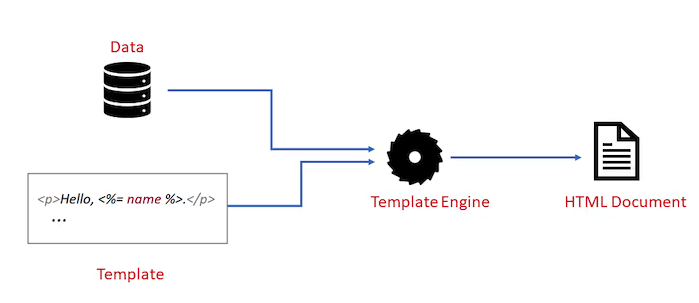
\includegraphics[scale=0.6]{imagens/modelo-ejs.png}}
\end{figure}

Os mecanismos de modelo lidam com a tarefa de interpolar dados em código HTML enquanto fornecem alguns recursos (como parciais em EJS) que seriam difíceis de replicar concatenando strings.

\subsection{Instalando e configurando o EJS}

Para instalar e configurar o EJS em nosso projeto, devemos, primeiramente, instalar a biblioteca que fornecerá o suporte em nossa aplicação e criar um diretório, na raiz do projeto, com o nome de \textbf{views}.

\begin{minted}[frame=single,framesep=10pt,breaklines,linenos,tabsize=2,autogobble]{javascript}
	yarn add ejs
	npm install ejs
\end{minted}

Agora, com a dependência já instalada, vamos configurar a nossa aplicação para usar o EJS. Isso tudo será feito dentro do nosso arquivo \textbf{index.js.}

\begin{minted}[frame=single,framesep=10pt,breaklines,linenos,tabsize=2,autogobble]{javascript}
	const express = require('express')
	const path = require('path');
	const app = express();
	const port = 3000
	
	app.use(express.static('public'));
	app.set('view engine', 'ejs');
	
	app.get('/', (req, res) => {
		res.render('index');
	})
	
	app.listen(port, () => {
		console.log(`Servidor executando na porta ${port}`)
	})
\end{minted}

E, no diretório \textbf{views}, criaremos um arquivo que será o utilizado para a exibição com o nome de \textbf{index.ejs}.

\subsection{Passando dados para serem renderizados}

Lembre-se de que nosso objetivo é combinar dados com modelos. Podemos fazer isso passando um segundo argumento para res.render. Este segundo argumento deve ser um objeto, que estará acessível no arquivo de modelo EJS.

Para tanto, adicione o seguinte código no arquivo \textbf{index.js}

\begin{minted}[frame=single,framesep=10pt,breaklines,linenos,tabsize=2,autogobble]{javascript}
	const express = require('express')
	const path = require('path');
	const app = express();
	const port = 3000
	
	app.use(express.static('public'));
	app.set('view engine', 'ejs');
	
	const usuario = {
		nome: 'Luiz',
		sobrenome: 'Picolo',
	}
	
	app.get('/', (req, res) => {
		res.render('index', {
			usuario
		})
	})
	
	app.listen(port, () => {
		console.log(`Servidor executando na porta ${port}`)
	})
\end{minted}

E no arquivo \textbf{index.ejs} inclua o objeto da seguinte forma:

\begin{minted}[frame=single,framesep=10pt,breaklines,linenos,tabsize=2,autogobble]{javascript}
	<h1>Olá, eu sou o <%= usuario.nome  %></h1>
\end{minted}

\subsection{Exercício de fixação}

1) Crie um rota de artigos. Depois, crie uma lista de postagens (como se fosse um blog) e liste-as ao acessar a rota artigos. Lembre-se de criar o arquivo EJS como feito anteriormente. 

\section{Requisições de objetos: req.params e req.query}

Até o momento, todos os dados que trafegaram em nossos estudos foram apenas do Servidor para o Cliente. Agora, a ideia é transmitir dados do Cliente para o Servidor. Para isso, vamos usar as três expressões descritas acima, req.body, req.query e req.params, que fazem parte do \textbf{Objeto de solicitação no Express.js} e são usados, pelo cliente, para enviar dados para o servidor. A princípio, vamos trabalhar com dados vindos das URLs.

\subsection{req.params}

O \textbf{req.params} tem com objetivo capturar propriedades anexadas ao URL, ou seja, parâmetros de rota nomeados. Você prefixa o nome do parâmetro com dois pontos (:) ao escrever suas rotas. Por exemplo, vamos capturar o parâmetro da URL abaixo:

\textbf{http://localhost:3000/artigos/123}

Assim, nossa rota artigos deve ser modificada da seguinte forma:

\begin{minted}[frame=single,framesep=10pt,breaklines,linenos,tabsize=2,autogobble]{javascript}
app.get('/artigos/:numero', (req, res) => {
	console.log(req.params.numero)
})	
\end{minted}

Caso houvesse mais parâmetros, poderíamos fazer da seguinte forma:

\textbf{http://localhost:3000/artigos/123/titulo}

\begin{minted}[frame=single,framesep=10pt,breaklines,linenos,tabsize=2,autogobble]{javascript}
	app.get('/artigos/:numero/:titulo', (req, res) => {
		console.log(req.params.numero)
		console.log(req.params.titulo)
	})	
\end{minted}

\subsection{req.query}

Já o req.query é usado principalmente para pesquisa, classificação, filtragem, paginação, etc. Digamos, que desejássemos obter a mesma URL anterior mas usando o query, ou, que tivessemos 10, 15 parâmetros. A escrita da rota ficaria comprometida pela dificuldade de entendimento. Assim, podemos rescrever tanto a \textbf{URL} como a \textbf{rota} ela usando o \textbf{req.query}. 

\textbf{http://localhost:3000/artigos?numero=123\&titulo=titulo-do-artigo}

\textbf{Observe com atenção}

Perceba que, após a rota é usando um ponto de interrogação, e, para separar os demais parâmetros, usando o \& também conhecido com E comercial.

\begin{minted}[frame=single,framesep=10pt,breaklines,linenos,tabsize=2,autogobble]{javascript}
	app.get('/artigos', (req, res) => {
		console.log(req.query.numero)
		console.log(req.query.titulo)
	})	
\end{minted}

\subsection{Exercício de Fixação}

1) A partir das URLs abaixo, crie suas respectivas rotas e, usando os conceitos aprendidos na aula anterior, apresente os parâmetros em um arquivos EJS.

\begin{itemize}[leftmargin=1.7cm]
	\setlength\itemsep{0em}
	\item http://localhost:3000/girafa?altura=15\&nome=juju
	\item http://localhost:3000/girafa/15/juju
	\item http://localhost:3000/noticias?id=123
	\item http://localhost:3000/noticias/123
\end{itemize}

2) Vamos usar as rotas para calcular o Teorema de Pitágoras. Use a seguinte URL para criar a rota e os parâmetros:

http://localhost:3000/pitagoras?a=4\&b=6\&c=3

\begin{figure}[H]
	\centering
	\frame{
\includegraphics[scale=0.6]{imagens/pitagoras.png}}
\end{figure}